% v2-acmlarge-sample.tex, dated March 6 2012
% This is a sample file for ACM large trim journals
%
% Compilation using 'acmlarge.cls' - version 1.3, Aptara Inc.
% (c) 2011 Association for Computing Machinery (ACM)
%
% Questions/Suggestions/Feedback should be addressed to => "acmtexsupport@aptaracorp.com".
% Users can also go through the FAQs available on the journal's submission webpage.
%
% Steps to compile: latex, bibtex, latex latex
%
\documentclass[prodmode,acmtap]{acmlarge}

%Metadata Information
\acmVolume{2}
\acmNumber{3}
\acmArticle{1}
\articleSeq{1}
\acmYear{2015}
\acmMonth{12}


% Package to generate and customize Algorithm as per ACM style
\usepackage[ruled]{algorithm2e}
\usepackage{caption}
\SetAlFnt{\algofont}
\SetAlCapFnt{\algofont}
\SetAlCapNameFnt{\algofont}
\SetAlCapHSkip{0pt}
\IncMargin{-\parindent}
\renewcommand{\algorithmcfname}{ALGORITHM}

% Page heads
% \markboth{D. Pineo, C. Ware and S. Fogarty}{Neural Modeling of Flow Rendering Effectiveness}

% Title portion
\title{What's cooking. STAT 841 final report.}
\author{Sajin Sasy and Alexandra Vtyurina \affil{University of Waterloo}
} 
% NOTE! Affiliations placed here should be for the institution where the
%       BULK of the research was done. If the author has gone to a new
%       institution, before publication, the (above) affiliation should NOT be changed.
%       The authors 'current' address may be given in the "Author's addresses:" block (below).
%       So for example, Mr. Fogarty, the bulk of the research was done at UIUC, and he is
%       currently affiliated with NASA.

\begin{abstract}
I CAN'T  WRITE THIS DAMN ABSTRACT!

\end{abstract}


\begin{document}

% \begin{bottomstuff}
% This work is supported by the Widget Corporation Grant \#312-001.\\
% Author's address: D. Pineo, Kingsbury Hall, 33 Academic Way, Durham,
% N.H. 03824; email: dspineo@comcast.net; Colin Ware, Jere A. Chase
% Ocean Engineering Lab, 24 Colovos Road, Durham, NH 03824; email: cware@ccom.unh.edu;
% Sean Fogarty, (Current address) NASA Ames Research Center, Moffett Field, California 94035.
% \end{bottomstuff}


\maketitle

% Head 1
\section{Introduction}

PROBLEM DESCRIPTON

INTRO

PAPER FLOW

\section{Data munging}
Kaggle provided all participants with two sets of data -- training and testing. Training data included almost 40 thousand recipes encoded as a list of json objects. Every recipe consisted of the following fields: \textit{id}, \textit{cuisine}, \textit{ingredients}. 20 different cuisines with 6714
%(without splitting, 3065 with splitting no stemming, 2692 with splitting and stemming) 
unique ingredients were presented in the training dataset. The test data had the same format with the exception of the \textit{cuisine} label, that should be predicted. The expected format of submission was a csv file with two columns - \textit{recipe id} and its predicted \textit{cuisine label}.

The training data provided was quite rich however unbalanced. \ref{cuisine_freq} shows how many recipes for each type of cuisine are contained in the training dataset. Underrepresented classes include brazilian, russian, jamaican, etc and contain under 800 recipes, whereas italian recipes dominate. 

It is worth mentioning the variability of the ingredients representation. Some only consisted of a single word (for ex. ``tomatoes''), whereas others contained multiple words (for ex. ``ground black pepper''). Moreover some ingredients also included attributes, such as ``2 large eggs'' and brand names ``Sargento® Traditional Cut Shredded Mozzarella Cheese''. This variability introduced additional noise to the data, and prevented us from using each ingredient as a separate feature. We further elaborate on the topic of data cleaning. 

\subsection{Data cleaning}
Given that ingredients may contain multiple words, using each ingredient as a separate feature will introduce a lot of noise, as “egg” and “eggs” will be considered two different features. Prior to classifying recipes, we cleaned the data in several different ways to see which one yields the best results and removes the most of noise. We chose different approaches, starting with a very mild one and building on top of one another to eventually reach the strictest cleaning strategy. 
We started off by splitting each ingredient into words\footnote{We used NLTK built in tokenizer to tokenization} and using them as features. This approach could deal with ingredients like ``large egg'' and ``egg'', splitting ``large egg'' into ``large'' and ``egg'', after which we had two ``egg'' terms match. 
But we still had problems in cases of ``three large eggs'' and ``egg'', where after splitting ``three large eggs'' into ``three'', ``large'', ``eggs'', the terms ``eggs'' and ``egg'' were still considered to be different. Stemming terms\footnote{We used Porter stemmer providd by NLTK} after splitting would solve this problem by transforming ``eggs'' into ``egg''. 

After examining the data we found that there are now ingredients that don’t add to the flavour of the dish, for example ``three'' and ``large'' (from ``three large eggs''), or ``ground'' and ``black'' (from ``ground black pepper''). Our assumption was that the main difference between cuisines comes from their flavour, hence only the ingredients themselves matter, rather than their modifiers. We wanted to remove modifiers based on the results of POS tagging (after manually examining the data we assumed that the majority of ingredients were nouns), but after performing POS tagging we found that the accuracy was extremely low due to the lack of context. E.g. we could only provide separate words and phrases to the tagger as opposed to entire sentences. As a result ingredients like ``store bought low sodium chicken broth'' the word ``store'' was considered a noun, even though it did not contribute to the flavour of the dish. Because of this issue we had to refuse from POS tagging and could not shrink initial data to bare ingredients. 


\begin{figure}[tp]
\centering
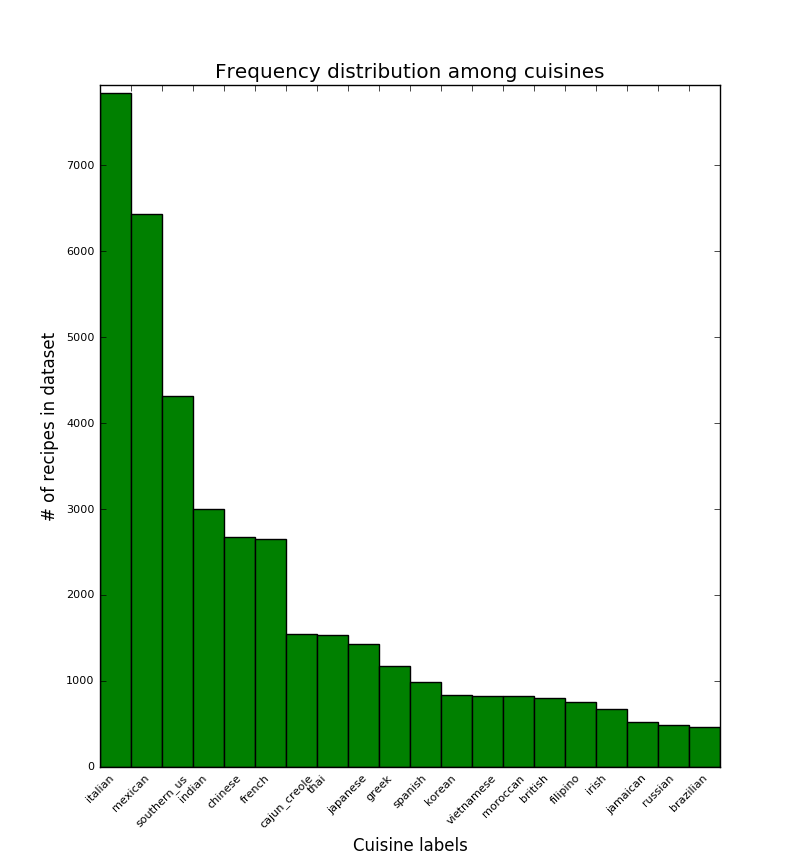
\includegraphics[scale=0.2]{cuisine_freq_hist_green_wlabels}
\caption{Training data is unbalanced. Italian and mexican recipes dominate, whereas brazilian and russian are underrepresented.}
\label{cuisine_freq}
\end{figure}

\section{Feature selection}
Mainly used bow
\subsection{PCA story}
After applying one-vs-one SVM to classify recipes we wanted to see how different the results would be for one-vs-all technique. For that we built 20\footnote{Same as the number of presented cuisines} hyperplanes to separate every single cuisine from the rest of the recipes. In this section we discuss our findings. 

First of all, to use one-vs-all approach we had to reduce the original problem to a binary classification problem. We did it by constructing a separate dataset for every given cuisine, where we changed labels to 1, in case the recipe belonged to the currently chosen cuisine, and 0 otherwise. For example, for separating italian recepies we created a dataset, where a label was 1, if the recipe was originally italian, and 0 otherwise. 

Having done that for each of the 20 cuisines we used 5-fold cross validation to evaluate the accuracy of the new model\footnote{Considering that we were looking at a single cuisine at a time, we could not submit to Kaggle to test the accuracy}. We found that even though the reported accuracy was very high (it varied from 94\% to 99\% for different cuisines), some recipes did not have any label by the end of the classification, which means they were not classified as positive for any of the cuisines. From that we can conclude the recall was low, e.g. the proposed model was failing to identify all the recipes from a given cuisine. 

We have also found that few of the recipes were classified as positive for multiple cuisines. Table \ref{confusiontable} shows the list of cuisines that were confused most often and the number of recipes that were positively classified multiple times. As seen in the table the cuisines that get misclassified also share geographical location and/or cultural features. 

\begin {table}
\centering
\begin{tabular}{|r|l||r|l|}
  \hline
  Confused cuisines & num of recipes & Confused cuisines & num of recipes \\
  \hline
  Thai and Vietnamese & 31 & Chinese and Korean & 14\\
  Southern US and Cajun creole & 28 & Italian and Greek & 11\\
  Italian and French & 25 & Indian and Moroccan & 9 \\
  \hline
\end{tabular}
\caption{Some of the recipes were classified as multiple cuisines. The table shows cuisines that were confused most often.}
\label{confusiontable}
\end {table}

After we found that some cuisines are hard for SVM to separate we looked at their recipes more closely and tried to find distinct features that could be used to differentiate the cuisines. We performed PCA on the recipes of Thai and Vietnamese cuisines. As showm in \ref{thai_taiwan_pca12}, the overlap between the two cuisines is quite large and the separation is more clear alomg the first principal component. 


\begin{figure}[tp]
\centering
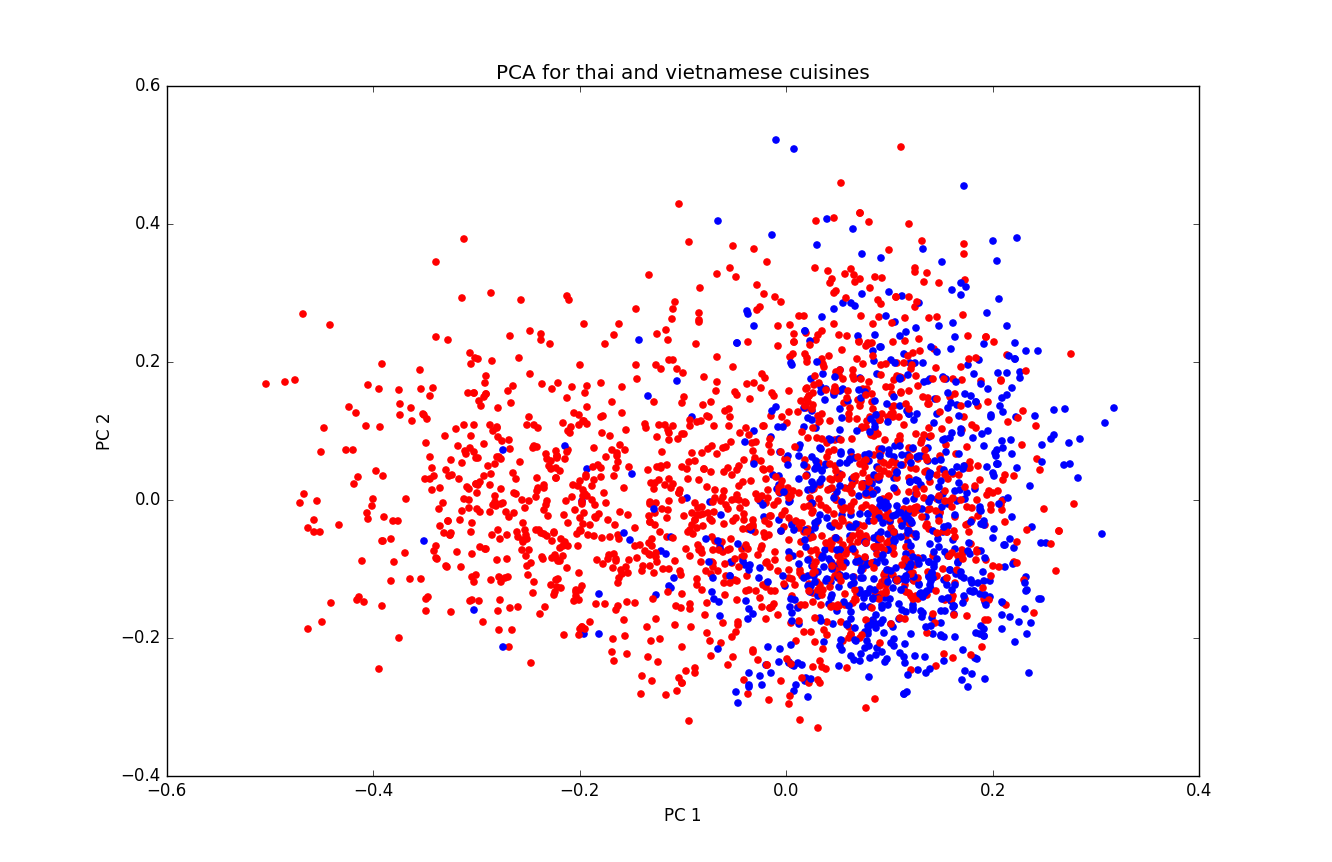
\includegraphics[scale=0.2]{PCA_thai_vietnam}
\caption{The first and the second principal components for recipes of Thai and Taiwanese cuisines.}
\label{thai_taiwan_pca12}
\end{figure}





\section{Classification approaches}
This part should be done. 

\section {Experiments}
I don't really know what to write here. Probs different results we got from different datasets. And why

\section{Discussion}
Future work and what not

\section{Conclusion}
We did that and it worked. 


% Bibliography
\bibliographystyle{ACM-Reference-Format-Journals}
\bibliography{acmlarge-sample-bibfile}
                                % Sample .bib file with references that match those in
                                % the 'Specifications Document (V1.5)' as well containing
                                % 'legacy' bibs and bibs with 'alternate codings'.
                                % Gerry Murray - March 2012

% History dates
% \received{February 2009}{July 2009}{October 2009}




\end{document}
% End of v2-acmlarge-sample.tex (March 2012) - Gerry Murray, ACM
